\setchapterstyle{kao}
\setchapterpreamble[u]{\margintoc}
\chapter{Structured sentence encoders at scale}
% using a generative objective
\labch{structure-scale}

% \section{Training efficient sentence embedding models using structured encoders}
% \labsec{structure-scale}

\cleanchapterquote{When people say AI has “learned x” what they usually mean is that a deep learning model has learned a dataset well enough to find the pattern you asked for. It has no symbolic or logical abstraction. It is kahnemann system 1. It looks smart. It isn’t.}{Mark Madsen}{Twitter post, 2019}

% The previous sections proposed to train sentence encoders at scale, In \refch{1B} by augmenting the pre-training corpus size and in \refch{generative} by proposing alternative pre-training objectives. In this section, we focus on the encoder architecture. We train various encoders and combine them in an original multi-view setup.




\bcomment{move after chap 5?}{}

\section{Motivation}
\labsec{structure:motivation}

% Inspired from linguistic insights, I assume structure is crucial to building consistent representations. I indeed expect sentence meaning to be a function of both syntax and semantic aspects. 
We hypothesize structure is a crucial element to perform compositional knowledge. In particular, the heterogeneity of performances across models and tasks makes us assume that some structures may be better adapted for a given example or task. Therefore, combining diverse structures should be more robust for tasks requiring complex word composition to derive their meaning. Hence, we aim here to evaluate the potential benefit from interactions between pairs of encoders. In particular, we propose a training method for which distinct encoders are learned jointly. We conjecture this association might improve our embeddings' power of generalization and propose an experimental setup to \bcomment{corroborate}{test} our hypothesis.

We take inspiration from multi-view learning, which is successfully applied in a variety of domains. In such a framework, the model learns representations by aligning separate observations of the same object. Such observations are referred to as \textit{views}. In our case, we consider a view for a given sentence as the association of the plain sentence with \bcomment{a syntactic structure}{several kinds of syntactic representations}. 

Combining different structural views has already been proven to be successful in many NLP applications. \textcite{kong_11} provide a heuristic to combine dependency and constituency analysis for coreference resolution. \textcite{zhou_16, ahmed_19_2} combine Tree LSTM and standard sequential LSTM with a cross-attention method and observe improvements on a semantic textual similarity task. \textcite{chen_liu_17} combine CNN and Tree LSTM using attention methods and outperform both models taken separately on a sentiment classification task. Finally, \textcite{chen_17} combine sequential LSTM and Tree LSTM for natural language inference tasks. 

The novelty here is to combine distinct structured models to build standalone sentence embeddings, which has not yet been explored. This paradigm benefits from several structural advantages. It pairs nicely with contrastive learning, as already mentioned. It \bcomment{might}{may} thus be trained in a self-supervised manner that does not require data annotation. Moreover, contrary to models presented in \bcomment{Section}{chapter} \ref{sec:multi-views}, our method is not specific to a certain kind of encoder architecture. It does not require, for example, the use of attention layers or tree-structured models.

Our setup could therefore be extended with any encoding function. Finally, our training method induces an interaction between models during inference and, paramountly, during the training phase.

\section{Method}
\labsec{structure:method}

\subsection{Contrastive learning}

\begin{figure*}[!htb]
\begin{center}
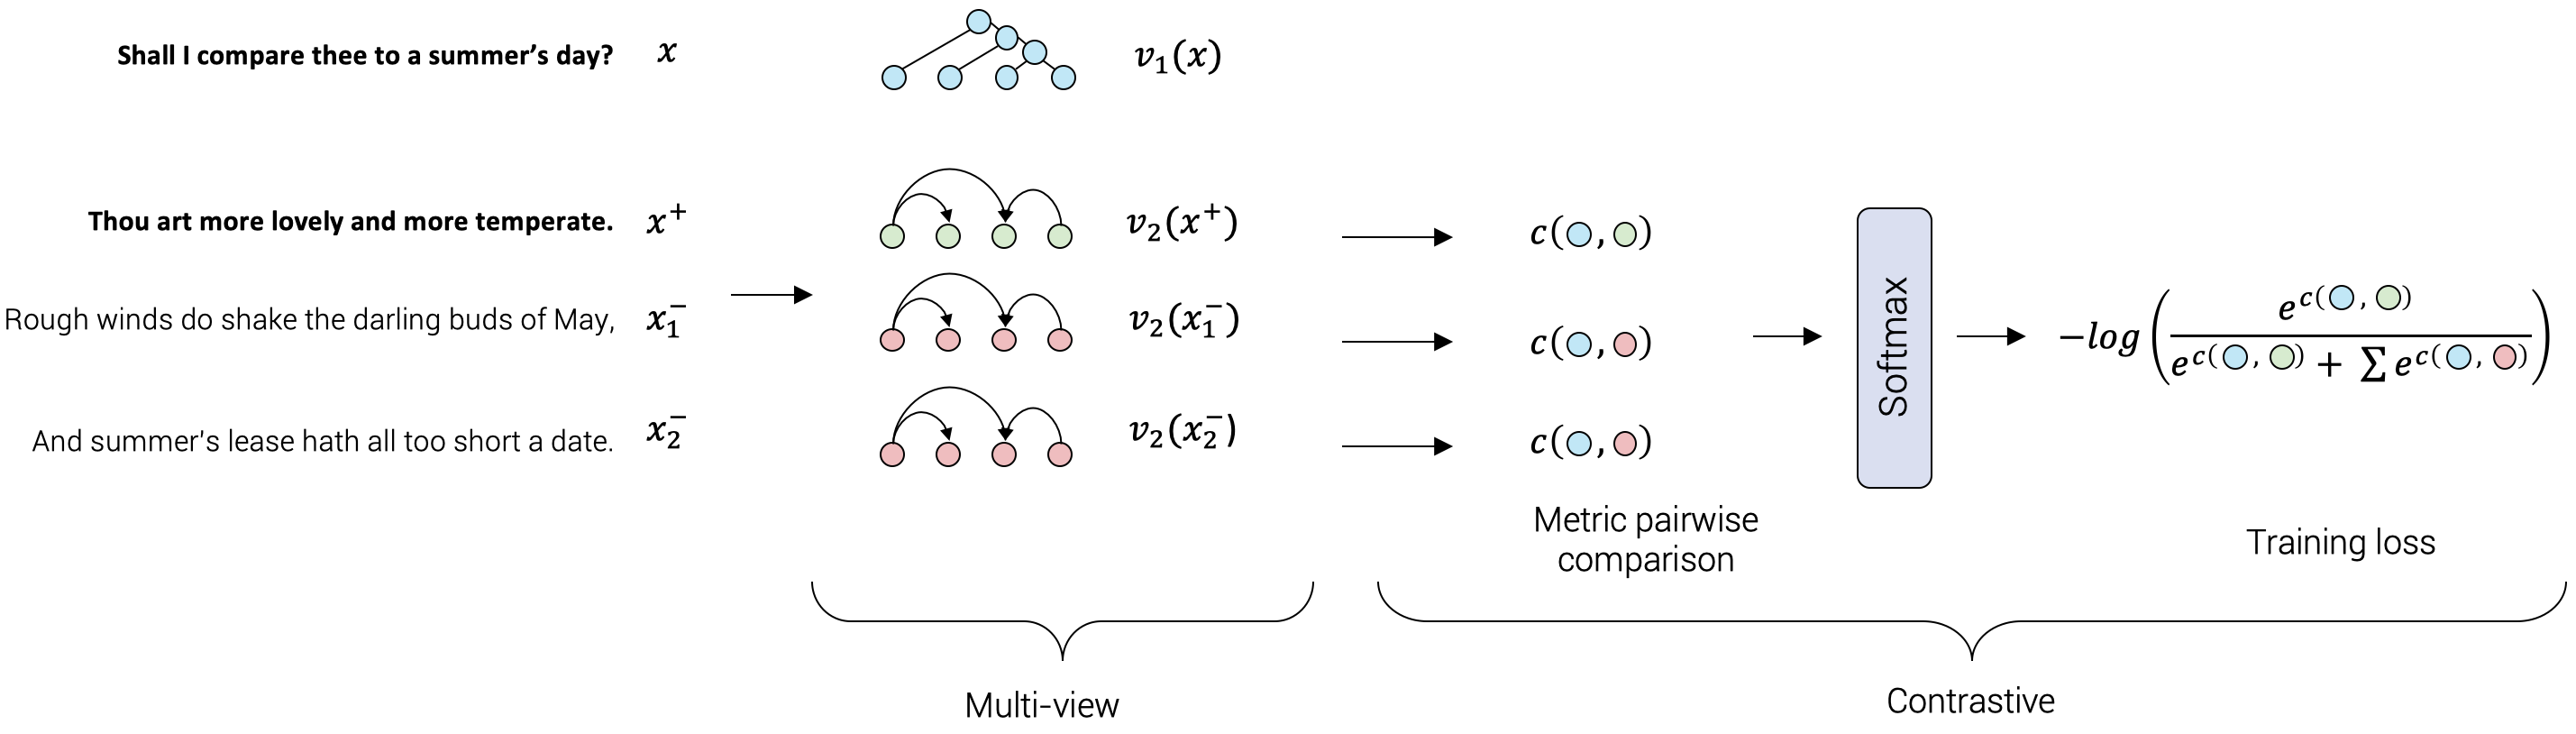
\includegraphics[width=15cm]{images/contrastive-4.png}
\end{center}
\caption{\textbf{Contrastive training method}. The objective is to reconstruct the storyline. Sentences are presented in their original order. Given an anchor sentence $x$, the model \bcomment{should}{has to} identify the context sentence $x^+$ out of negative samples $x_1^-, x_2^-$. Sentences are encoded using separate views, which are composed within a pairwise distance matrix. }
\labfig{contrastive}
\end{figure*}

We train our model using the contrastive objective from \textcite{logeswaran_18}, detailed in \refsec{training}. The method takes inspiration from the distributional hypothesis successfully applied for \bcomment{word}{words}, but this time, to identify context sentences. Given a sentence $s$, a corresponding context sentence $s^+$ and a set of $K$ negative samples $s^-_1 \cdots s^-_K$, the training objective is to maximize the probability of \bcomment{discriminate}{predicting} the correct sentence among negative samples: $p(s^+ | S)$ with $S = \{s, s^+, s^-_1 \cdots s^-_K\}$. As illustrated in \reffig{contrastive}, two sentences encoders $f$ and $g$ are defined and the conditional probability is estimated as follow\footnote{\citet{logeswaran_18} simply use an inner product for $c$ such as $c\left(x, y\right) = x^Ty$. In our case, as the encoders $f$ and $g$ are distincts, we choose a bilinear function defined as $c\left(x, y\right) = x^TWy$ \cite{tschannen_20}.}:

\[
p(s^+ | S) = \frac{e^{c\left(f(s), g(s^+)\right)}}{e^{c\left(f(s), g(s^+)\right)}+\sum_{i=1}^Ne^{c\left(f(s), g(s^-_i)\right)}}
\]

At inference time, the sentence representation is obtained as the concatenation of the two encoders $f$ and $g$ such as $s \rightarrow [f(s);g(s)]$, as illustrated in \reffig{inference}. In \textcite{logeswaran_18}, $f$ and $g$ use the same RNN encoder. However, the authors observe that the encoders might learn redundant features. To limit this effect, they propose to use a distinct set of embeddings for each encoder. 

We propose addressing this aspect by enhancing the method with a multi-view framework and using a distinct structured model for the encoders $f$ and $g$. We hypothesize that some structures may be better adapted for a given example or task. 
For example, dependency parsing usually sets the verb as the root node. Whereas in constituency parsing, subject and verb are often the right and left child from the root node. Therefore, the combination of different structures should be more robust for tasks requiring complex word composition and be less sensitive to lexical variations. Consequently, we propose a training procedure that allows the model to benefit from the interaction of various syntactic structures.

\subsection{Language views}

Multi-view aims as learning representations from data represented by multiple independent sets of features. We generalize the notion of view for a sentence as the application of a specific syntactic framework. For each view, we use an \textit{ad-hoc} algorithm that maps the structured sentence into an embedding space.

We consider structures exposed in \refsec{survey:encoding}: Vanilla GRU (\textsc{Seq}), dependency tree combined with the Child-Sum Tree LSTM (\textsc{Dep}), Constituency tree combined with N-Ary Tree LSTM (\textsc{Const}). Although \bcomment{under some hypotheses}{}equivalences might be derived between the \bcomment{last}{} two representations schemes, we hypothesize that, in our context, the corresponding sequence of operations might allow capturing rather distinct linguistic properties. The various models may, therefore, be complementary and their combination allows for more fine-grained analysis. 

For the \textsc{Dep} view, the dependency tree is obtained using the deep biaffine parser from \textcite{dozat_17}. We use an open-source implementation\sidenote{\url{https://github.com/yzhangcs/biaffine-parser}} of the dependency parser \parencite{dozat_17} and replace the pos-tags features with features obtained with \textsc{bert}. Therefore we do not need pos-tags annotations to parse our corpus. Regarding the inference speed, The constituency parser is the bottleneck in this case and parse around 500 sentences/second. In our case, the parsing of the entire corpus (40M sentences) take about a day to complete. 

For the \textsc{Const} view, the structure is obtained using the constituency neural parser from \textcite{klein_18}. We binarize the trees to ensure that every node has exactly two dependents. The binarization is performed using a \bcomment{left markovization}{add ref} and unary productions are collapsed in a single node. 

\begin{figure}[!htb]
\begin{center}
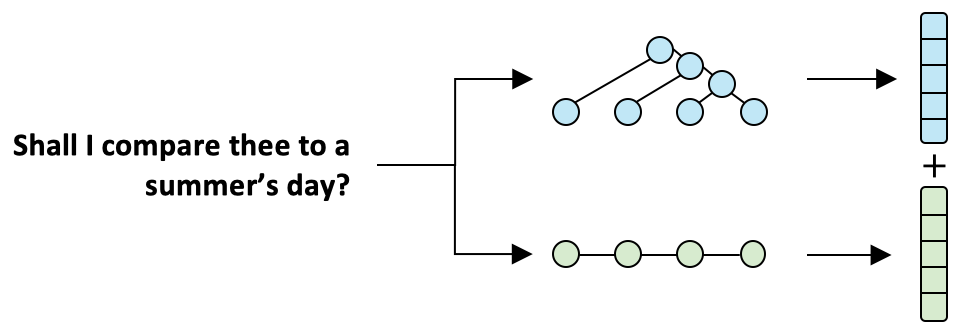
\includegraphics[width=10cm]{images/contrastive-inf.png}
\end{center}
\caption{\textbf{Multi-view sentence embedding}. At inference, embeddings are the concatenation from both views.}
\labfig{inference}
\end{figure}

\section{Experiments}
\labsec{structure:experiments}

We train our models on the UMBC dataset \footnote{\url{https://ebiquity.umbc.edu/blogger/2013/05/01/umbc-webbase-corpus-of-3b-english-words/}}\sidenote{The bookcorpus introduced in \textcite{zhu_15} and traditionally used for sentence embedding is no longer distributed for copyright reasons. Therefore, we prefer a corpus freely available. The impact of the training dataset choice is analyzed in Appendix \ref{appendix:training-dataset}.} \parencite{han_13}. We limited our corpus to the first 40M sentences from the tokenized corpus. Indeed, \textcite{logeswaran_18} already analyze the effect of the corpus size, and we focus here on the impact of our multi-view setting. We build batches from successive sentences. \bcomment{Given a sentence in a batch, other sentences not in the context are considered as negatives samples}{slightly unclear}. 

Model hyper parameters are fixed given literature on comparable work \parencite{tai_15, logeswaran_18}. All models are trained using a batch size of 400 and the Adam optimizer with a $5e^{-4}$ learning rate. Regarding the infrastructure, we use a Nvidia GTX 1080 Ti GPU. All model weights are initialized with a Xavier distribution and biases set to 0. We do not apply any dropout. 

For the vocabulary, we follow the setup proposed in \textcite{kiros_15, logeswaran_18} and we train two models in each configuration. One initialized with pre-trained embedding vectors. The vectors are not updated during training and the vocabulary includes the top 2M cased words from the 300-dimensional GloVe vectors\sidenote{\url{https://nlp.stanford.edu/projects/glove/}} \parencite{pennington_14}. The other is limited to 50K words initialized with a Xavier distribution and updated during training. For inference, the vocabulary is expanded to 2M words using a linear projection.

\subsection{Evaluation on SentEval}

\begin{table*}[!htb]
\footnotesize
% \begin{minipage}{\textwidth}
\centering {
\begin{tabularx}{16cm}{@{}c c Y | Y Y Y Y Y Y Y Y Y Y @{}}
\toprule
\multirow{2}{*}{\textbf{Model}} & \multirow{2}{*}{\textbf{Dim}} & \multirow{2}{*}{\textbf{Hrs}} & \multirow{2}{*}{\textbf{MR}} & \multirow{2}{*}{\textbf{CR}} & \multirow{2}{*}{\textbf{SUBJ}} & \multirow{2}{*}{\textbf{MPQA}} & \multirow{2}{*}{\textbf{TREC}} &  \multicolumn{2}{c}{\textbf{MRPC}} &  \multicolumn{3}{c}{\textbf{SICK-R}}\\%\cmidrule(r){9-10} \cmidrule(r){11-13}
 &  &  &  &  &  &  &  & \textbf{Acc} & \textbf{F1} & \textbf{$r$} & \textbf{$\rho$} & \textbf{MSE}\\\midrule
\multicolumn{13}{c}{\textit{Context sentences prediction}} \\\midrule
FastSent & $\leq500$ & 2 & 70.8 & 78.4 & 88.7 & 80.6 & 76.8 & 72.2 & 80.3 & --- & --- & ---\\
FastSent + AE & $\leq500$ & 2 & 71.8 & 76.7 & 88.8 & 81.5 & 80.4 & 71.2 & 79.1 & --- & --- & ---\\
Skipthought & $4800$ & 336 & 76.5 & 80.1 & 93.6 & 87.1 & 92.2 & 73.0 & 82.0 & 85.8 & 79.2 & 26.9\\
Skipthought + LN & $4800$ & 672 & 79.4 & 83.1 & 93.7 & 89.3 & --- & --- & --- & 85.8 & 78.8 & 27.0\\
Quickthoughts & $4800$ & 11 & \textbf{80.4} & \textbf{85.2} & \textbf{93.9} & \textbf{89.4} & \textbf{92.8} & \textbf{76.9} & \textbf{84.0} & \textbf{86.8} & \textbf{80.1} & \textbf{25.6}\\
\midrule\multicolumn{13}{c}{\textit{Sentence relations prediction}} \\\midrule
InferSent & $4096$ & --- & \textbf{81.1} & \textbf{86.3} & 92.4 & 90.2 & 88.2 & \textbf{76.2} & \textbf{83.1} & \textbf{\underline{88.4}} & --- & ---\\
DisSent Books 5 & $4096$ & --- & 80.2 & 85.4 & 93.2 & 90.2 & 91.2 & 76.1 & --- & 84.5 & --- & ---\\
DisSent Books 8 & $4096$ & --- & 79.8 & 85.0 & \textbf{93.4} & \textbf{\underline{90.5}} & \textbf{\underline{93.0}} & 76.1 & --- & 85.4 & --- & ---\\
\midrule\multicolumn{13}{c}{\textit{Pre-trained transformers}} \\\midrule
\textsc{Bert}-base [CLS] & $768$ & 96 & 78.7 & 84.9 & 94.2 & 88.2 & \textbf{91.4} & 71.1 & --- & 75.7$^\dagger$ & --- & ---\\
\textsc{Bert}-base [NLI] & $768$ & 96 & \textbf{\underline{83.6}} & \textbf{\underline{89.4}} & \textbf{94.4} & \textbf{89.9} & 89.6 & \textbf{76.0} & --- & \textbf{84.4}$^\dagger$ & --- & ---\\
\midrule\multicolumn{13}{c}{\textit{\textbf{Our models (GloVe \& Pretrained Embeddings)}}} \\\midrule
\textsc{Seq}, \textsc{Const}$^\dagger$ & $4800$ & 41 & 79.8 & 82.9 & 94.6 & 88.5 & 90.4 & 76.4 & 83.7 & 86.1 & 78.9 & 26.3\\
\textsc{Dep}, \textsc{Seq}$^\dagger$ & $4800$ & 27 & 79.7 & 82.2 & 94.4 & 88.6 & 91.0 & \textbf{\underline{77.9}} & \textbf{\underline{84.4}} & 86.6 & 79.8 & 25.5\\
\textsc{Dep}, \textsc{Const}$^\dagger$ & $4800$ & 39 & \textbf{80.7} & \textbf{83.6} & \textbf{\underline{94.9}} & \textbf{89.2} & \textbf{92.6} & 76.8 & 83.6 & \textbf{87.0} & \textbf{\underline{80.3}} & \textbf{\underline{24.8}}\\
\bottomrule
\end{tabularx}}
\caption{\textbf{SentEval Task Results Using Fixed Sentence Encoder.} 
We divided the table into sections. The first range of models is directly comparable to our model as the training objective is to identify context sentences. The second section objective is to identify the correct relationship between a pair of sentences. The third section reports pre-trained transformers based-models. The last section reports the results from our models. FastSent is reported from \textcite{hill_16}. Skipthoughts results from \textcite{kiros_15} Skipthoughts + LN which includes layer normalization method from \textcite{ba_16}. We considered the Quickthoughts results \cite{logeswaran_18} with a pre-training on the bookcorpus dataset. DisSent and Infersent are reported from \textcite{nie_19} and \textcite{conneau_17} respectively. Pre-trained transformers results are reported from \textcite{reimers_19}. The \textbf{Hrs} column indicates indicative training time, the \textbf{Dim} column corresponds to the sentence embedding dimension. $^\dagger$\, indicates models that we had to re-train. Best results in each section are shown in \textbf{bold}, best results overall are \underline{underlined}. Performance for \textbf{SICK-R} results are reported by convention as $\rho \text{ and } r \times 100$.}
\labtab{contrastive-soa}
\end{table*}

As usual for models aiming to build generic sentence embeddings \textcite{kiros_15, hill_16, arora_17, conneau_17, logeswaran_18, nie_19}, we use tasks from the SentEval benchmark \parencite{conneau_18}\sidenote{Senteval is posterior to most of the references. However, these studies do evaluate on tasks later included in the benchmark.}. SentEval is specifically designed to assess the quality of the embeddings themselves rather than the quality of a model specifically targeting a downstream task, as is the case for the GLUE and SuperGLUE benchmarks \parencite{wang_19_glue, wang_19_superglue}. Indeed, the evaluation protocol prevents for fine-tuning the model during inference and the architecture to tackle the downstream tasks is kept minimal. Moreover, the embedding is kept identical for all tasks, thus assessing their properties of generalization. 

Therefore, classification tasks from the SentEval benchmark are usually used for evaluation of sentence representations \parencite{conneau_18}: the tasks (presented in \refsec{survey:downstream}) include sentiment and subjectivity analysis (\textbf{MR, CR, SUBJ, MPQA}), question type classification (\textbf{TREC}), paraphrase identification (\textbf{MRPC}) and semantic relatedness (\textbf{SICK-R}). Contrasting the results of our model on this set of tasks will help to better understand its properties.  The MR, CR, SUBJ, MPQA tasks are binary classification tasks with no pre-defined train-test split. We therefore use a 10-fold cross validation. For the other tasks we use the proposed train/dev/test splits.
%We use either the pre-defined train/dev/test splits or perform a 10-fold cross-validation. 
We follow the linear evaluation protocol of \textcite{kiros_15}, where a logistic regression or softmax classifier is trained on top of sentence representations. The dev set is used for choosing the regularization parameter and results are reported on the test set. 

% \paragraph{Results analysis} 

We compare the properties of distinct views combination on downstream tasks. Results are compared with state of the art methods in \reftab{contrastive-soa}. The first set of methods (\textsl{Context sentences prediction}) are trained to reconstruct books storyline. % relies on a distributional hypothesis: models 
The second set of models (\textsl{Sentence relations prediction}) is pre-trained on a supervised task. Infersent \parencite{conneau_17} is trained on the SNLI dataset, which proposes to predict the entailment relation between two sentences. DisSent \parencite{nie_19} proposes a generalization of the method and builds a corpus of sentence pairs with more possible relations between them. Finally, we include models relying on transformer architectures (Pre-trained transformers) for comparison. In particular, \textsc{Bert}-base model and a \textsc{Bert}-model fine-tuned on the SNLI dataset \cite{reimers_19}. 
In \reftab{contrastive-soa}, we observe that our models expressing a combination of views such as (\textsc{Dep}, \textsc{Seq} or (\textsc{Dep}, \textbf{const}) give better results than the use of the same view (\textbf{seq}, \textbf{seq}) used in Quick-Thought model. It seems that the entanglement of views benefits the sentence embedding properties. In particular, we obtain state-of-the-art results for almost every metric from \textbf{MRPC} and \textbf{SICK-R} tasks, which focus on paraphrase identification. For the \textbf{MRPC} task, we gain a full point in accuracy and outperform \textsc{Bert} models. We hypothesize structure is important for achieving this task, especially as the dataset is composed of rather long sentences. The \textbf{SICK-R} dataset is structurally designed to discriminate models that rely on compositional operations. 

This also explains the score improvement on this task. Tasks such as \textbf{MR}, \textbf{CR} or \textbf{MPQA} consist in sentiment or subjectivity analysis. We hypothesize that our models are less relevant in this case: such tasks are less sensitive to structure and depend more on individual word or lexical variation.

\subsection{Impact of the multi-view}
\labsec{impact-multi-view}

We aim to measure the impact of multi-view specifically. Table~\ref{table:multi-view} compares all possible view pairs out of \textsc{Dep}, \textsc{Const} and \textsc{Seq} views. For each multi-view model, we report the average score from SentEval tasks\sidenote{We scale all metrics as percentages. In particular, we use 100 - MSE for the \textbf{SICK-R} task. The final score corresponds to the average of all tasks. We average the scores for tasks with multiple metrics (\textbf{MRPC} and \textbf{SICK-R}).}. The first section of the Table corresponds to \textit{single-view} models, for which both views from the pair are identical. The second section reports multi-view models. 

Multi-view models outperform those using a single view. Given our experiment, it is advantageous to use multiple views instead of one. It also confirms our hypothesis that combining multiple structured models or views yield richer sentence embeddings.

\begin{table}[!htb]
\footnotesize
% \begin{minipage}{\textwidth}
\centering {
\begin{tabularx}{\textwidth}{@{}c | Y@{}}
\toprule
Model & Avg. SentEval Score \\\midrule
\multicolumn{2}{c}{\textit{Single-view models}} \\\midrule
\textsc{Const}, \textsc{Const} & 84.4\\
\textsc{Dep}, \textsc{Dep} & 84.6\\
\textsc{Seq}, \textsc{Seq} & 84.9\\\midrule
\multicolumn{2}{c}{\textit{Multi-view models}} \\\midrule
\textsc{Seq}, \textsc{Const} & 85.1\\
\textsc{Seq}, \textsc{Dep} & 85.3\\
\textsc{Dep}, \textsc{Const} & \textbf{86.0}\\
\bottomrule
\end{tabularx}}
\caption{\textbf{Impact of the multi-view.} The first section corresponds to single-view setups for which $f$ and $g$ are the same views. The second section reports multi-view models. For each model, we report the average score on the SentEval benchmark.}
\label{table:multi-view}
\end{table}

\subsection{Impact of the corpus choice}
\labsec{impact-corpus}

We have chosen to make use of a distinct corpus as the BookCorpus dataset is no longer distributed for copyright reasons. We have run QuickThought scripts \parencite{logeswaran_18} using our dataset based on the UMBC corpus to compare both setups. Results are detailed in the first Section from \reftab{corpus} and are rather close in both configurations. Indeed, except for the \textbf{SUBJ} and \textbf{MR} task, the use of our dataset penalizes the results. Our corpus is indeed restricted to 40M sentences, in comparison with 74M for the Bookcorpus. Regarding the dataset size and the SentEval results, we have considered the comparison holds.

\begin{table*}[!htb]
\footnotesize
% \begin{minipage}{\textwidth}
\centering {
\begin{tabularx}{16cm}{@{}c| Y Y Y Y Y Y Y Y Y Y @{}}
\toprule
\multirow{2}{*}{\textbf{Model}} & \multirow{2}{*}{\textbf{MR}} & \multirow{2}{*}{\textbf{CR}} & \multirow{2}{*}{\textbf{SUBJ}} & \multirow{2}{*}{\textbf{MPQA}} & \multirow{2}{*}{\textbf{TREC}} &  \multicolumn{2}{c}{\textbf{MRPC}} &  \multicolumn{3}{c}{\textbf{SICK-R}}\\%\cmidrule(r){9-10} \cmidrule(r){11-13}
 &  &  &  &  &  & \textbf{Acc} & \textbf{F1} & \textbf{$r$} & \textbf{$\rho$} & \textbf{MSE}\\\midrule
 \multicolumn{11}{c}{\it Impact of the pretraining corpus on QuickThought} \\\midrule
Quickthoughts (results from paper) & 80.4 & \textbf{85.2} & 93.9 & \textbf{89.4} & \textbf{92.8} & \textbf{76.9} & 84.0 & \textbf{86.8} & \textbf{80.1} & \textbf{25.6}\\
Quickthoughts (UMCB 40M)$^\dagger$ & \textbf{80.9} & 84.4 & \textbf{95.1} & 88.9 & 92.2 & 75.8 & --- & 86.0 & --- & ---\\\midrule
 \multicolumn{11}{c}{\it Impact of the embedding size} \\\midrule
{\sc Bert}-base [CLS] $^\dagger$& \textbf{77.3} & 81.3 & 92.7 & 85.0 & 80.2 & 69.9 & --- & 61.0 & --- & ---\\
{\sc Bert}-base [CLS] /w random projection $^\dagger$& 77.1 & \textbf{82.6} & \textbf{93.1} & \textbf{85.9} & \textbf{80.8} & \textbf{71.3} & --- & \textbf{71.0} & --- & ---\\\midrule
 \multicolumn{11}{c}{\it Impact of pre-training}\\\midrule
\dep{}, \const{}$^\dagger$ & \textbf{80.7} & \textbf{83.6} & \textbf{94.9} & \textbf{89.2} & \textbf{92.6} & \textbf{76.8} & \textbf{83.6} & \textbf{87.0} & \textbf{80.3} & \textbf{24.8}\\
Rand \sc{LSTM} & 77.2 & 78.7 & 91.9 & 87.9 & 86.5 & 74.1 & --- & 86.0 & --- & ---\\
\bottomrule
\end{tabularx}}
\caption{\labtab{corpus}Study on SentEval task results: the first section compares the impact of the training dataset for QuickToughts. The next section focuses on the impact of the embedding size. To this end, hidden representations are projected into a larger embedding space using a random, fully connected layer. The final Section compares models randomly initialized with those pre-trained on our self-supervised task. $^\dagger$ indicates models that we had to re-train.}
\end{table*}

\bcomment{as it stands this table remains slightly mysterious : how do we compare with table 9.2 ? + with your best results + put the embedding size+what is the random projection + missing line model}{}

\subsection{Biases toward embedding size}
\labsec{impact:embedding-size}

As exposed in \refsec{training:supervised}, SentEval evaluation framework is suspected to suffers from biases toward the embedding size \parencite{eger_19}. Moreover, some works on sentence embedding evaluation methods points surprising good results may be achieved using randomly initialized encoders \parencite{wieting_19}. We provide extra analysis to discuss these potential pitfalls.

Regarding the dependency on the embedding size, we run experiments to analyze if such bias could explain \textsc{Bert} low performances on SentEval since the output hidden size is only of $768$. Following the protocol from \textcite{wieting_19}, we project the embedding from the \textsc{CLS} token using a random matrix initialized with a glorot distribution. This setup expands \textsc{Bert} embedding into 4096 dimensions. We reported the results in \reftab{corpus}. We observe expanding the embedding size seems to slightly improve the results. However, the results are still below Quickthought vectors by a large margin.

Regarding the effect of randomly initialized encoders \parencite{wieting_19}, we reported the results in \reftab{corpus}. Although randomly initialized encoders achieve surprisingly good results, they are still below our results obtained with pre-training.

\section{Conclusion and future work}

Inspired from linguistic insights and supervised learning, we hypothesize that structure is a central element to build sentence embeddings. The novelty here is detailed in \refsec{structure:method} and consists in jointly learning structured models in a contrastive framework. In \refsec{structure:experiments} we evaluate the standalone sentence embeddings and use them as a feature for the dedicated SentEval benchmark. We obtain state-of-the-art results on tasks which are expected, by hypothesis, to be more sensitive to sentence structure. We show in \refsec{impact-multi-view} that multi-view embeddings yield better downstream task results. Our \bcomment{setup}{result} confirms our hypothesis that combining diverse structures should be more robust for tasks requiring to perform complex compositional knowledge.